\documentclass[11pt]{article}

\usepackage[top=1.5in, bottom=1.5in, left=1in, right=1in]{geometry}

\usepackage[lined, boxed, linesnumbered]{algorithm2e}
\usepackage[Sonny]{fncychap}
\usepackage{fancyhdr}
\usepackage{graphicx}
\usepackage{multirow}
\usepackage{verbatim}
\usepackage{float}
\usepackage{longtable}
\usepackage{pdfpages}
\usepackage{listings}
\usepackage{amsmath}
\usepackage{url}

\usepackage{parskip}

\begin{document}
\centerline{\bf \Large UniID\footnote{Replace UniID with your University ID and remove this footnote.}: Adversarial Search Evaluation}
\bigskip

It is good practise to have a brief introductory paragraph describing your evaluation approach and main findings.

{\bf Important:} Note that you {\em should not} introduce the Connect game or the minimax algorithm. You may assume that the reader has good knowledge of the coursework. The report should focus on the {\em evaluation} of minimax and minimax with alpha-beta pruning. Similarly, you should not discuss implementation details unless these are strictly relevant to the evaluation.

As discussed in the coursework document, you might consider how the methods perform individually and how they compare to each other.

It is up to you how you structure your report, but it should be {\bf 3 pages} in length {\em using this template}. Any additional pages, with the exception of references, will be ignored. The remainder of this template is a suggested structure, but you are free to modify this.

\section{Evaluation of Minimax without pruning}

As discussed in the coursework document, aspects you may discuss include the impact of the size of the board, the number of pieces required to be in a line to win, the overheads of the methods, etc. When performing the evaluation you should consider that different runs may get different results, and so you may wish report details such as the mean and standard deviation for the metrics you discuss. You may want to include a table of results, such as Table~\ref{table:1} or a plot of results such as Fig.~\ref{figure:example}.

\begin{table}[h!]
\centering
\begin{tabular}{c | c c c} 
 Experiment & Metric 1 & Metric 2 & Metric 3 \\ 
 \hline
 1 & 3 & 26 & 3 \\ 
 2 & 65 & 45 & 346 \\
 3 & 55 & 53 & 5 \\
 4 & 3455 & 242 & 67 \\
 5 & 328 & 87 & 44 
\end{tabular}
\caption{Example table.}
\label{table:1}
\end{table}

\begin{figure}[!ht]
\centering
\caption{Example figure.}
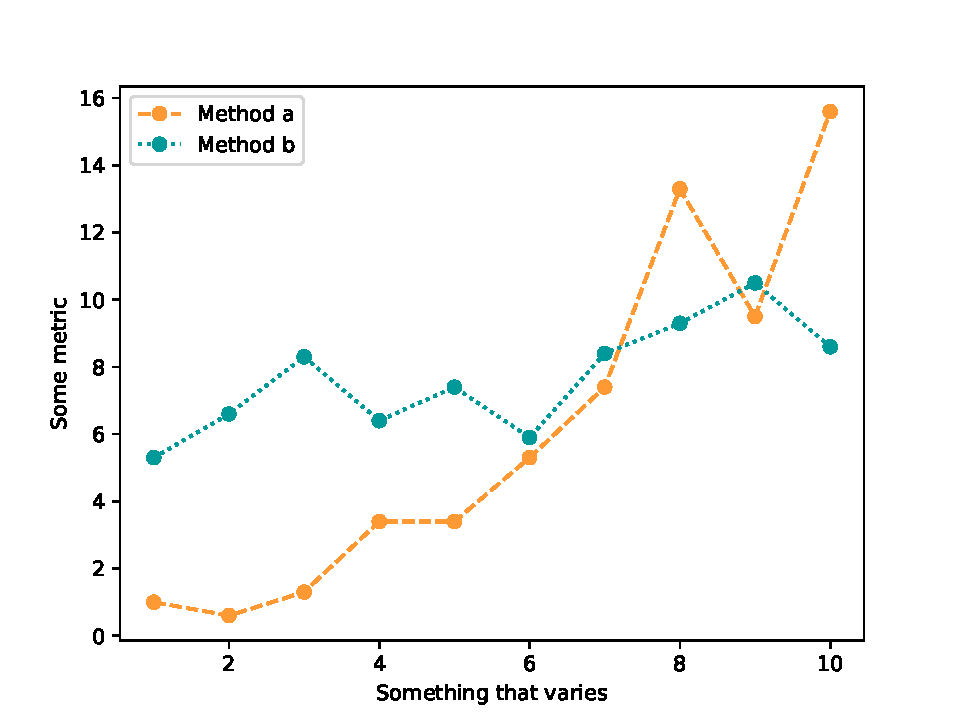
\includegraphics[width=0.4\textwidth]{figure_example.pdf}
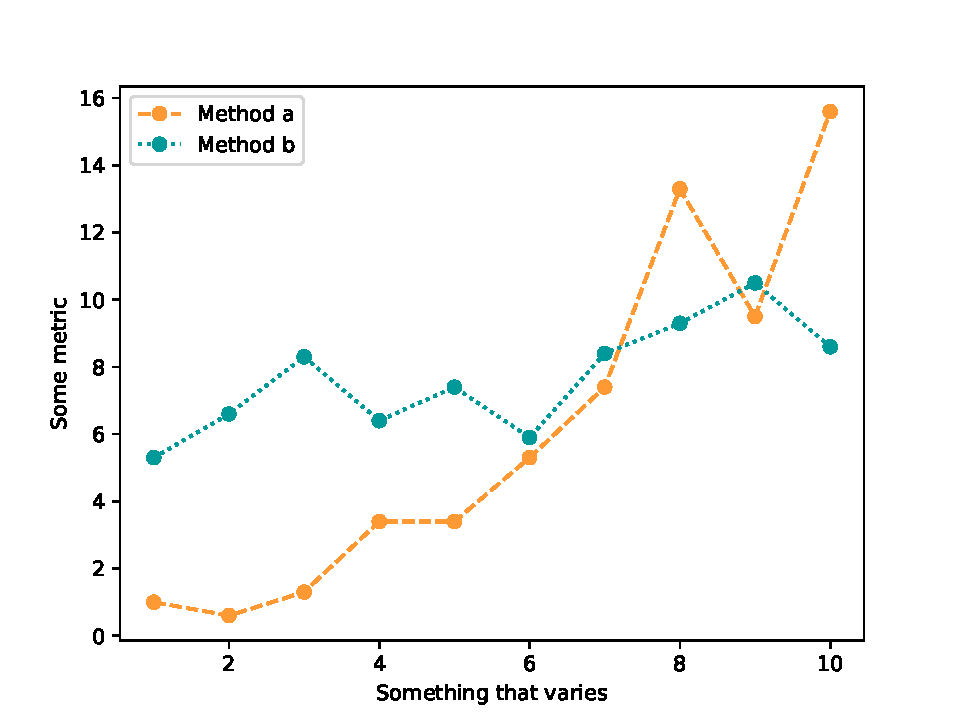
\includegraphics[width=0.4\textwidth]{figure_example.pdf}
\label{figure:example}
\end{figure}

\section{Evaluation of Minimax with alpha-beta pruning}

\section{Discussion and Conclusions}

\section{References}

Although not required, you might want to use Bibtex for your references. If you are not familiar with Bibtex, there is a good introduction at \url{https://www.overleaf.com/learn/latex/Bibliography_management_with_bibtex}.

\end{document}